\subsection{Применение АКФ для компенсации шума}

Для эффективного использования АР-метода необходимо иметь точную оценку АКФ. Наличие шума в аддитивной смеси ведет к неточной
оценке АКФ ведет к смещенной оценке резонансных частот. Увеличение ОСШ при вычислении АКФ зависит, в том числе от длительности
выборки. В тех случаях длинну выборки увеличить не представляется возможным, например в случае обработки в реальном времени,
возникает необходимость искать другие способы повышения ОСШ.

В подобных случаях в \cite{ostanin_akf} предлагяется использовать метод последовательного вычисления АКФ. Данный метод
заключается в последовательном вычислении АКФ от АКФ несколько раз. При этом ОСШ увеличивается от итерации к итерации.
Процесс повторяется несколько раз. Количество итераций зависит от среднего значения ОСШ сигнала. Очевидно, что
для СНС сигналов ОСШ для приемника ниже, чем для сигналов систем сотовой связи.

Пусть исходный сигнал может быть записан как сумма полезного сигнала ${x(t)}$ и шума ${n(t)}$:
\begin{center}
\begin{equation}
	\label{eq:acf_signal}
	s(t) = A \cos{(\omega t)} + n(t)
\end{equation}
\end{center}

Пусть функции ${s(t)}$ и ${n(t)}$ - центрированы. Тогда АКФ выражения \ref{eq:acf_signal} может быть записан как \cite{book_max}:
\begin{center}
\begin{eqnarray}
	\label{eq:acf_rss_signal}
	r_{ss}(\tau)	& = & \lim_{T \to \infty} \frac{1}{T} \int \limits_0^T s(t)s(t-\tau)dt = \nonumber \\
			& = & \lim_{T \to \infty} \frac{1}{T} \int \limits_0^T (A \cos{(\omega t)} + n(t))(A \cos{(\omega t - \tau)} + n(t - \tau))dt
\end{eqnarray}
\end{center}

Тогда, оценка АКФ может быть записана как:
\begin{center}
\begin{equation}
	\label{eq:acf_rss_signal_full}
	\hat{r}_{ss}(\tau)=\hat{r}_{xx}(\tau)+\hat{r}_{xn}(\tau)+\hat{r}_{nx}(\tau) + \hat{r}_{nn}(\tau)
\end{equation}
\end{center}

АКФ шума стремится к 0 с увеличением длинны выборки. Длинна выборки при которой ${\hat{r}_{nn}(t)}$ становится нулем зависит от характеристик шума.
Корреляционные функции ${\hat{r}_{xn}}$ и ${\hat{r}_{nx}}$ тождественно равны 0, с точностью до погрешности, при условии независимости
${x(t)}$ и ${n(t)}$. Таким образом \ref{eq:acf_signal} можно переписать:
\begin{center}
\begin{equation}
	\label{eq:acf_rss_signal_new}
	\hat{r}_{ss}(t) = \hat{r}_{xx}(t) + \epsilon (t)
\end{equation}
\end{center}
Стоит учесть, что ${\epsilon (t)}$ стремится к нулю с ростом ${T}$. В \cite{ostanin_akf} отмечено, что Фурье-образ ${\hat{r}_{xx}(t)}$
представляет собой СПМ, а следовательно равен квадрату Фурье-образа исходной функции ${x(t)}$.
Если обозначить ОСШ, выраженное в линейных единицах, сигнала ${s(t)}$ как ${R_s}$, тогда ОСШ после вычисления АКФ может быть вычислено
как \cite{book_max}:
\begin{center}
\begin{equation}
	\label{eq:acf_snr_est}
	R_e=2BTR_s \frac{1}{2+1/R_s}
\end{equation}
\end{center}

Стоит отметить, что функция ${\epsilon(\tau)}$, как и ${n(t)}$ - является центрированной и
стационарной случайной величиной.
Учитывая что гармоническая составляющая содержится в ${\hat{r}_{ss}(t)}$, а аддитивный шум в ${\epsilon(\tau)}$, можно провести
следующую итерацию вычисления АКФ. Для оценки ОСШ по формуле \ref{eq:acf_snr_est} нужно принять ${R_s' = R_e}$.

Из \ref{eq:acf_snr_est} видно, что увеличение ОСШ при вычислении оценки АКФ пропорционально ${2BT}$ и зависит от
ОСШ на входе коррелометра, так же можно отметить, что увеличение ОСШ происходит только при условии ${BT > \frac{1}{2R_s} + 1}$.

Так же можно получить оценку АКФ на ${N}$ - шаге. На рисунке \ref{pic:acf_0_iter} представлен входной сигнал, а на
риcунках \ref{pic:acf_1_iter}, \ref{pic:acf_4_iter} представлены оценки АКФ на шагах с 1 и 4.
Моделирование проводилось для гармонического сигнала при ОСШ -44 дБ с нормированной частотой 20 Гц для
отрезка 600 точек.

\begin{figure}[H]
	\center\scalebox{1}{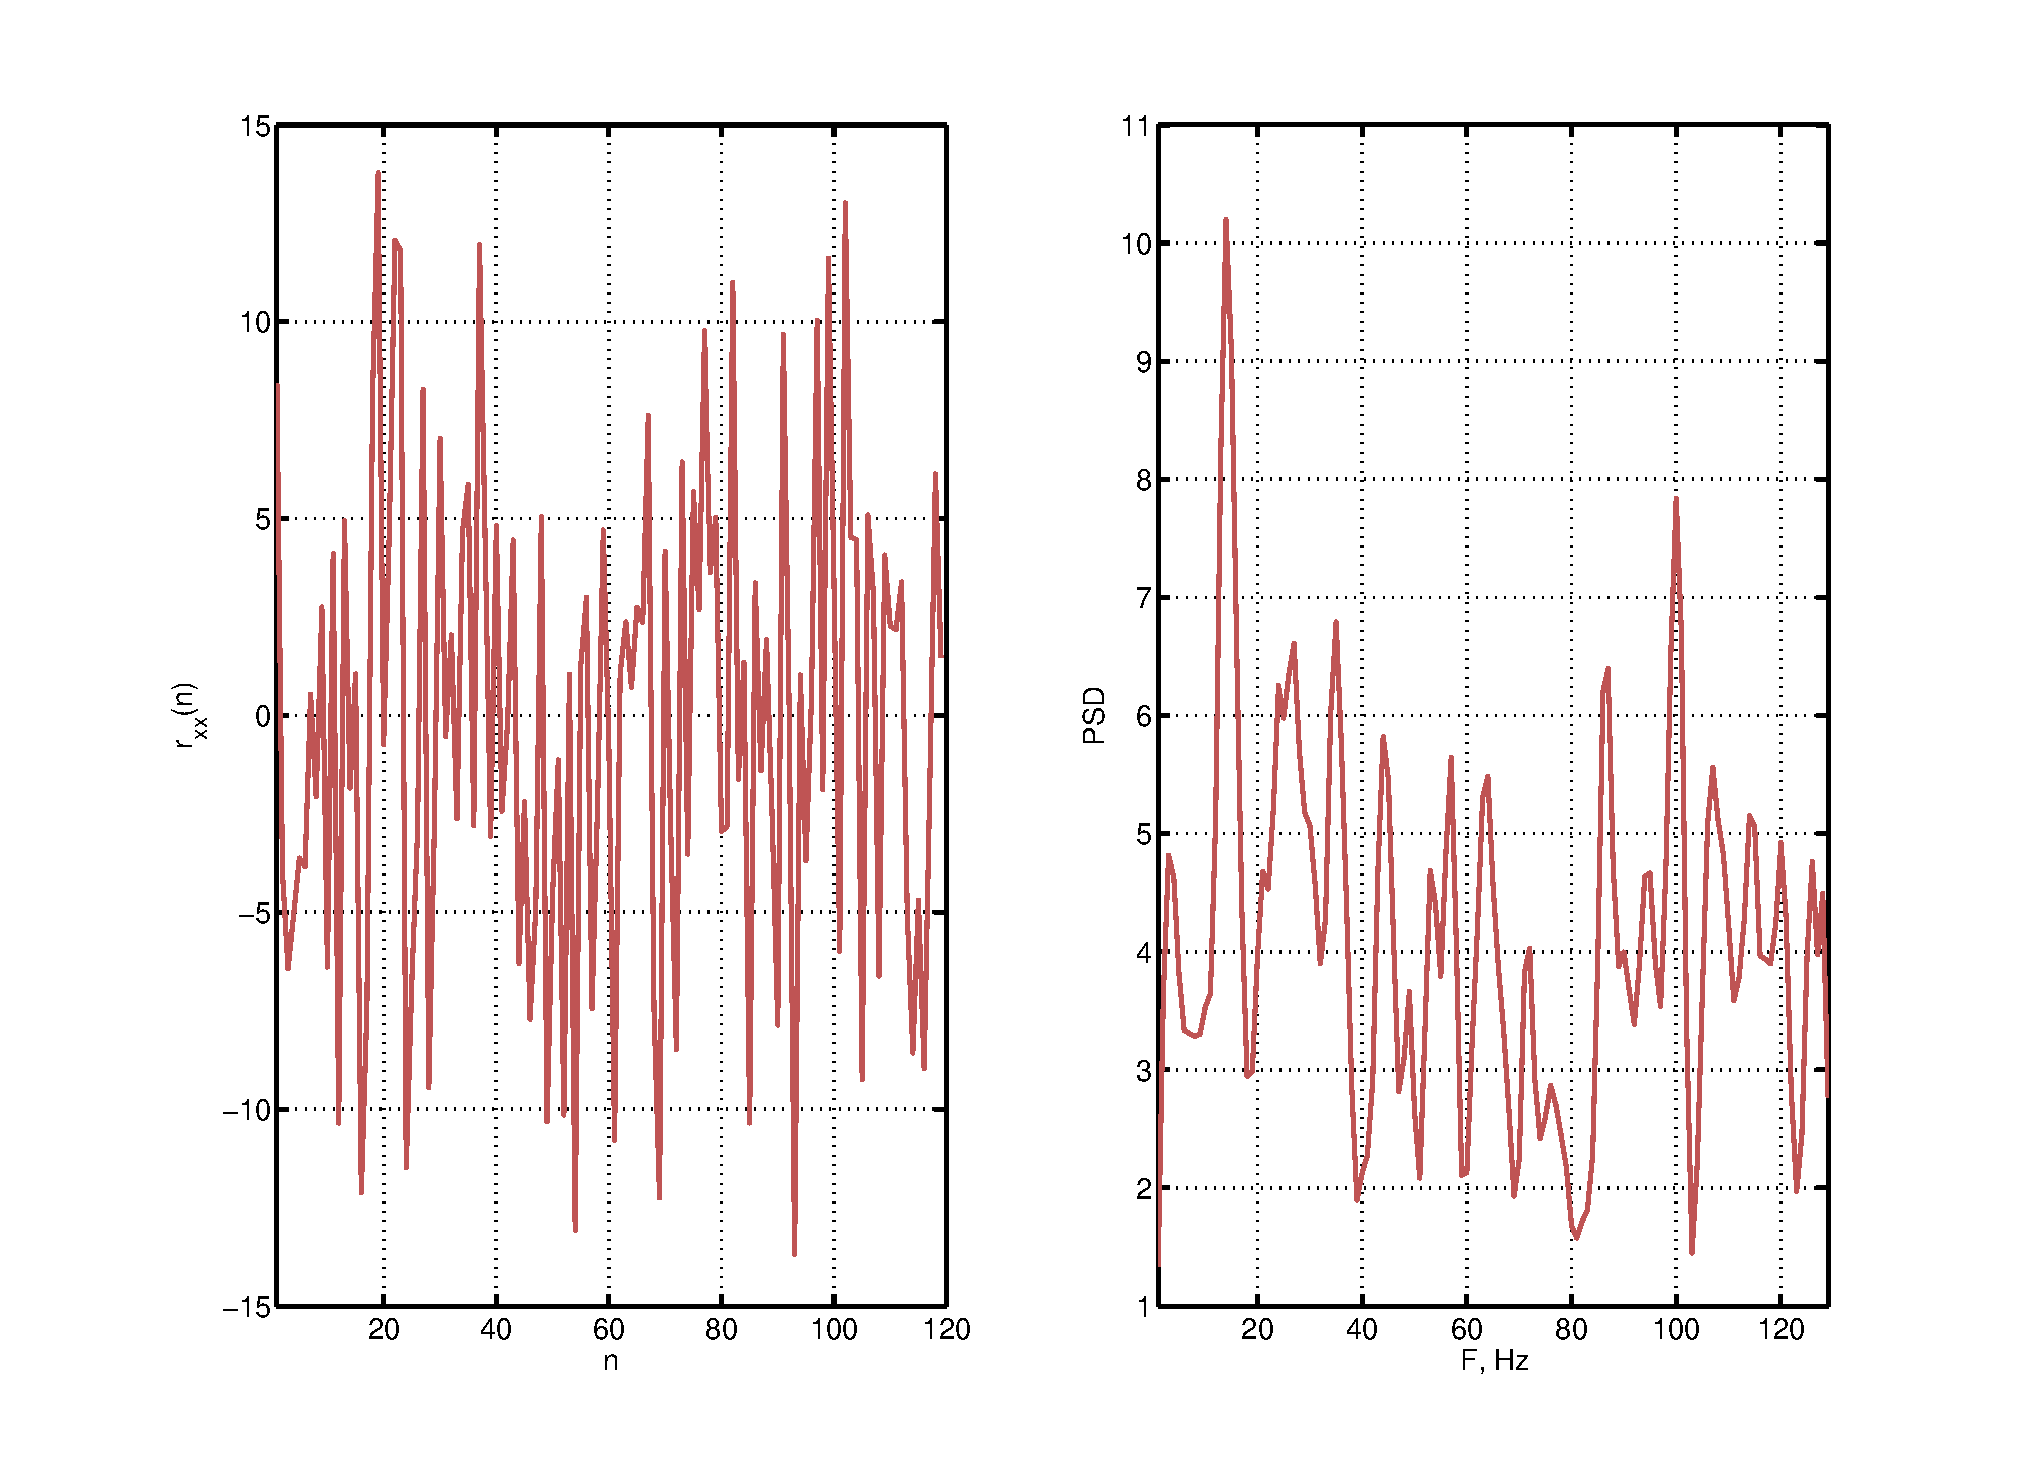
\includegraphics[width=1\linewidth]{acf_0_iter.eps}}
	\caption{Исходный сигнал и его спектр.}
	\label{pic:acf_0_iter}
\end{figure}

\begin{figure}[H]
	\center\scalebox{1}{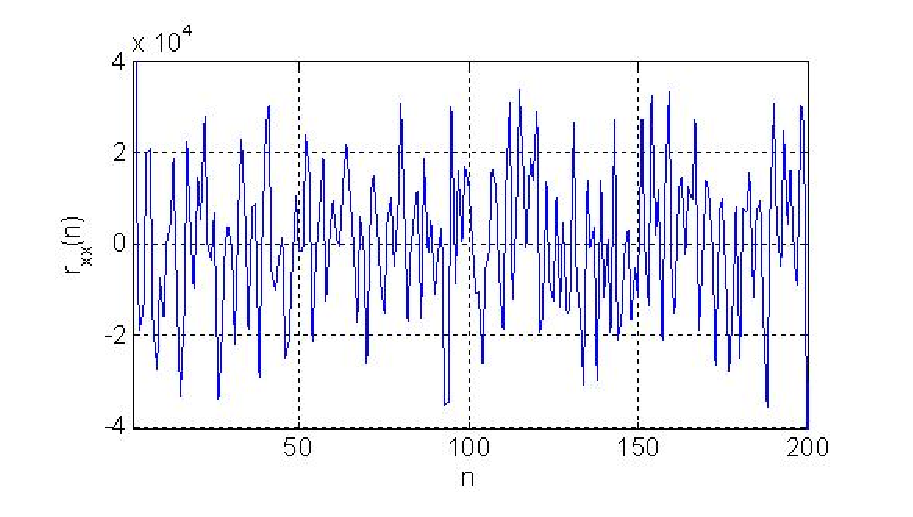
\includegraphics[width=1\linewidth]{acf_1_iter.eps}}
	\caption{Оценка АКФ на 1 итерации и ее спектр.}
	\label{pic:acf_1_iter}
\end{figure}

\begin{figure}[H]
	\center\scalebox{1}{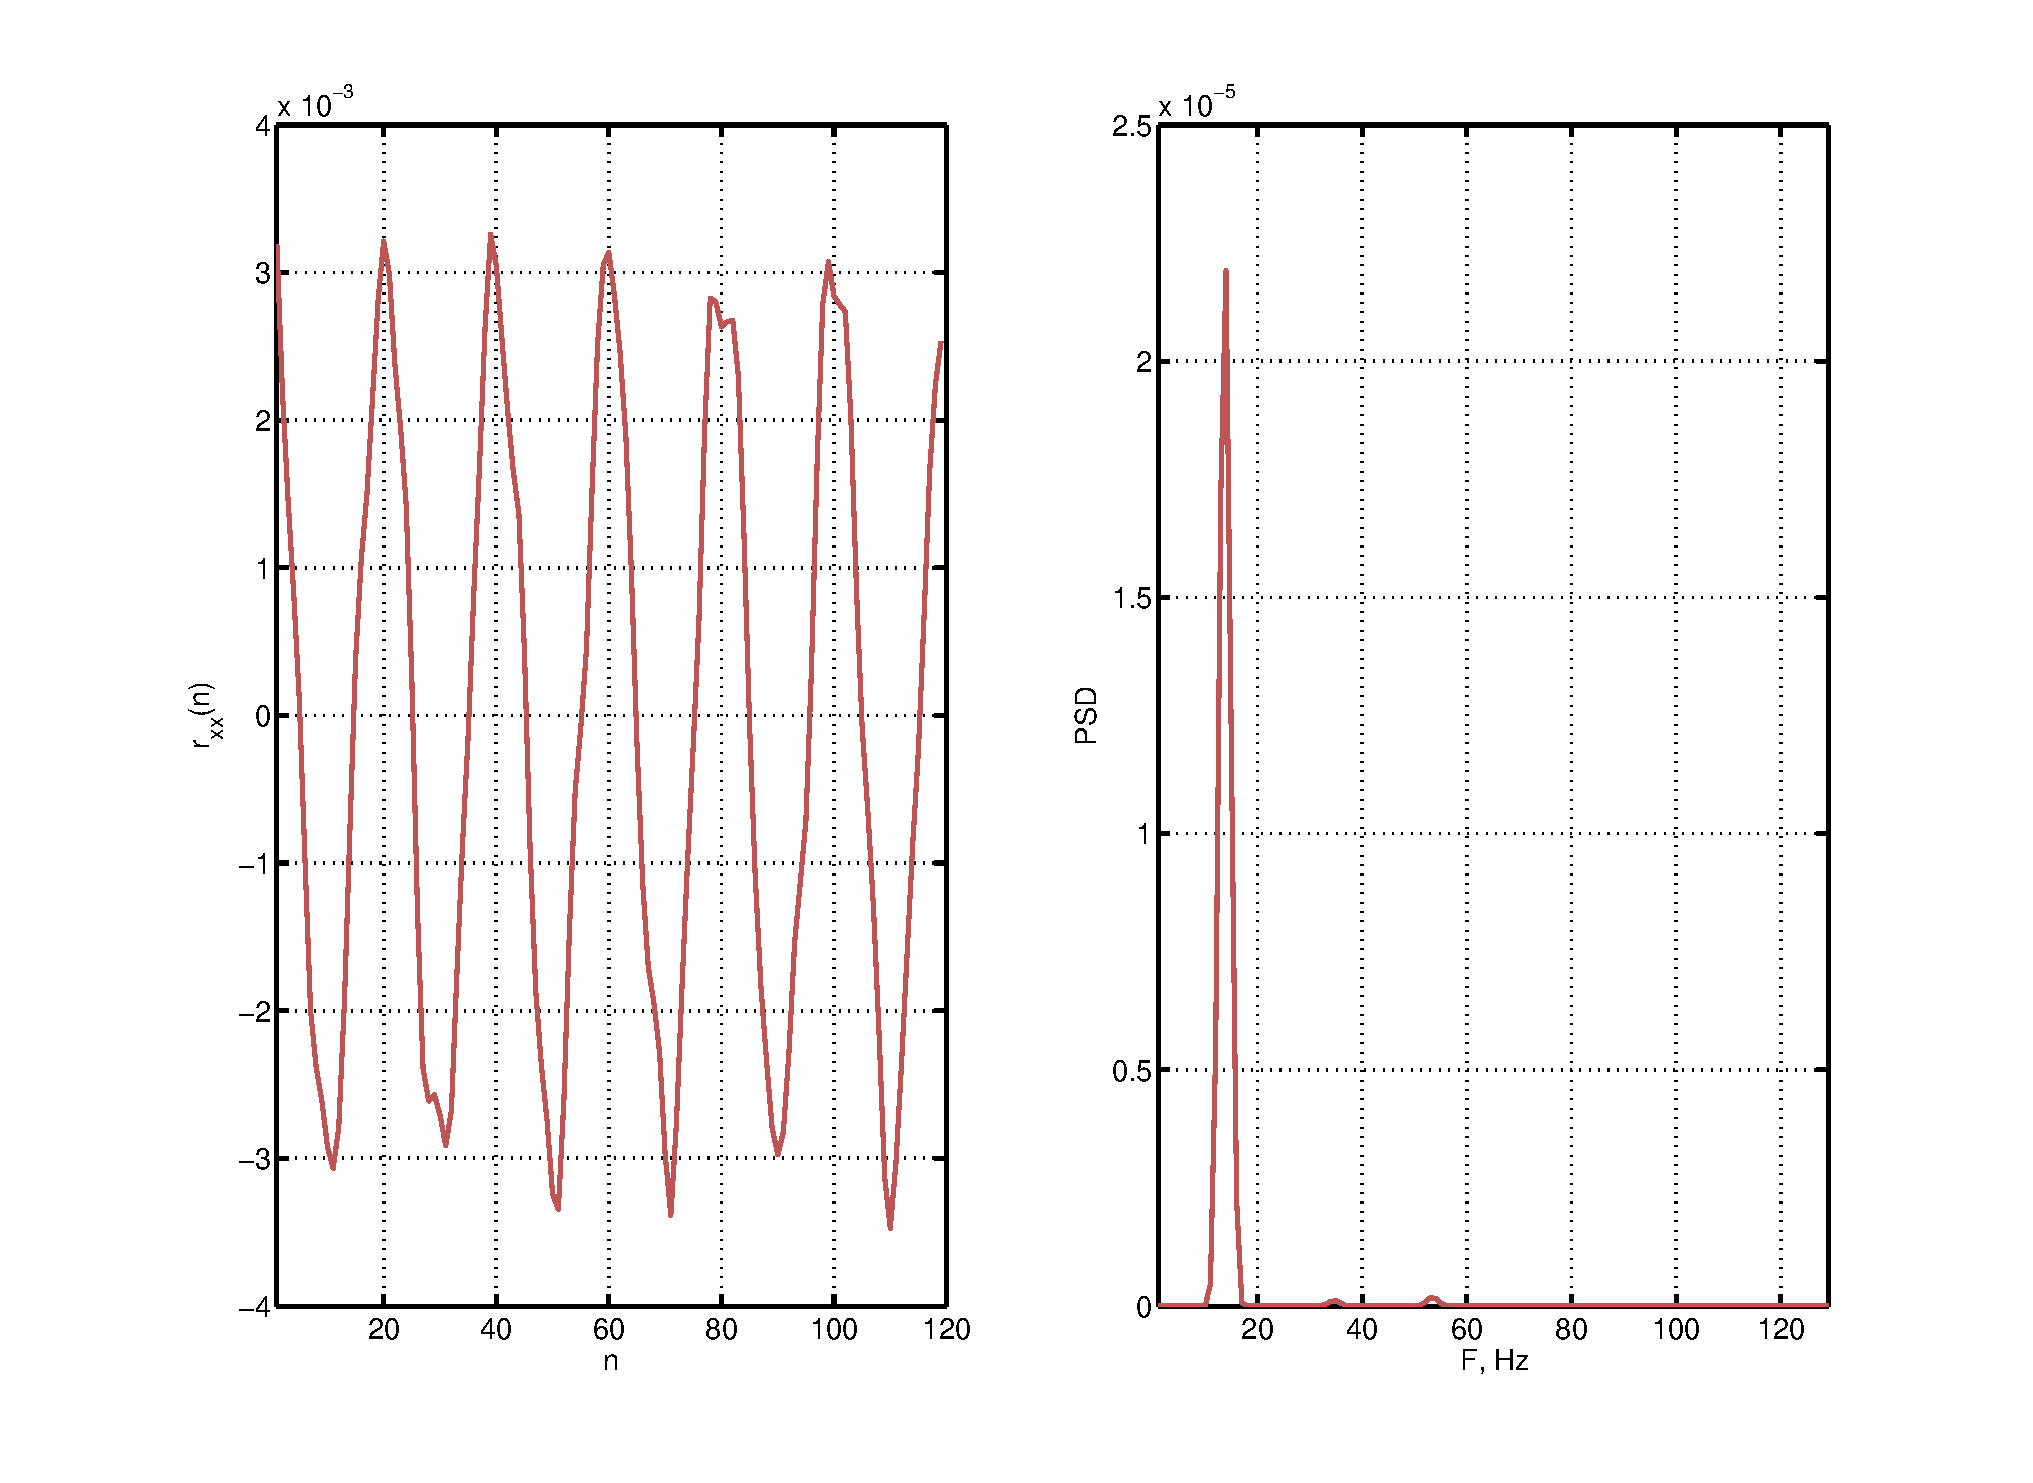
\includegraphics[width=1\linewidth]{acf_4_iter.eps}}
	\caption{Оценка АКФ на 4 итерации и ее спектр.}
	\label{pic:acf_4_iter}
\end{figure}
``
\newpage
